% !TeX root=../main.tex

\chapter{روش پیشنهادی}
%\thispagestyle{empty} 
\section{مقدمه} 
در این فصل به توضیح مبانی نظری روش پیشنهادی پرداخته می‌شود. روش پیشنهادی شامل یک عملگر قابل آموزش با فرمول بندی شبیه \lr{LBP} و قرار دادن این عملگر در لایه اول شبکه کانولوشن کلاسیک است. از آنجا که در مسئله کشف تقلب به‌جای تمرکز روی ویژگی‌های ظاهری نظیر گوشه‌ها، لبه‌ها و... اطلاعات بافت تصاویر اهمیت دارد این لایه مبتنی بر \lr{LBP} پیشنهاد شده است. 
ابتدا عملگر \lr{LBP} قابل آموزش بیان خواهد شد. سپس ساختار شبکه تشریح خواهد شد و در ادامه به توضیح تابع هزینه معرفی شده پرداخته می‌شود. 

برای بیان عملگر \lr{LBP} قابل آموزش ابتدا توضیحی کلی از عملگر کانولوشن و شبکه‌های کانولوشنی همراه با شهود استفاده از این شبکه‌ها در مسائل بینایی ماشین، بیان خواهد شد. سپس رابطه ریاضی عملگر کانولوشن و عملگر \lr{LBP} ارائه شده و با همانندسازی این دو عملگر، عملگر \lr{LBP} قابل آموزش به‌دست خواهد آمد.
در ادامه برای بهینه کردن شبکه با هدف بهبود دقت و افزایش قابلیت تعمیم‌پذیری، دو تابع هزینه معرفی خواهد شد. در تابع هزینه اول هدف تفکیک کردن دو کلاس با حاشیه است و در تابع هزینه دوم هدف مجبور کردن شبکه به توجه به ویژگی‌های تقلب به‌جای توجه به ویژگی‌های ظاهری افراد است.
\section{مروری بر عملگر کانولوشن}
یکی از اجزای اصلی شبکه‌های مبتنی بر یادگیری عمیق عملگر کانولوشن است. این عملگر دارای یک هسته‌ی ضرایب است که به‌صورت پیچشی در تصویر ورودی ضرب می‌شود و سپس با لغزش بر کل تصویر ورودی، یک تصویر خروجی به‌دست خواهد آمد. 

اعمال عملگر کانولوشن روی سیگنال معادل ضرب تبدیل فوریه عملگر در تبدیل فوریه تصویر ورودی است و با این ضرب می‌توان برخی از فرکانس‌های تصویر ورودی را تقویت یا تضعیف کرد که فیلتر کردن تصویر ورودی خواهد بود. اعمال وزن‌های مختلف به هسته فیلتر می‌تواند خروجی تصویر با مشخصات خاصی را بدهد.

برای مثال با استفاده از وزن‌های خاص در عملگر می‌توان یک فیلتر پایین‌گذر طراحی کرد و با اعمال عملگر کانولوشن این فیلتر پایین‌گذر، یک تصویر که فرکانس‌های بالای آن حذف شده‌اند به‌دست آورد. طراحی فیلترهای مختلف برای اهداف گوناگونی نظیر یافتن لبه در تصویر یا حذف نویز تصویر می‌تواند کاربرد داشته باشد. اما هر هدف نیازمند یک فیلتر خاص از قبل طراحی شده است. 

ایده شبکه‌های عصبی کانولوشنی
\LTRfootnote{Convolutional neural network} (\lr{CNN}) 
در این است که وزن‌های فیلتر به‌صورت پارامتر در نظر گرفته شود و در طی فرآیند بهینه‌سازی تابع هزینه، ضرایب فیلتر به‌روزرسانی شوند و فیلترهای مد نظر از طریق داده‌های موجود به‌دست آیند. 
هر اعمال یک لایه کانولوشن روی تصویر باعث به‌دست آوردن ویژگی‌ها جدید می‌شود و با اعمال متوالی عملگر پارامتری شده کانولوشن، ویژگی‌های مفهومی‌تر به‌دست خواهد آمد. این ساختار لایه‌ای در صورتی که با تعداد کافی داده، بهینه شود می‌تواند ویژگی‌های معنایی از تصویر را استخراج کند. که این دریافت معنا از تصویر باعث کاربردهای مختلفی نظیر طبقه‌بندی، تشخیص شئ، شناسایی چهره و... شده است.

در مسئله تشخیص تقلب در تشخیص چهره، بیش از آنکه ویژگی‌های معنایی تصویر مد نظر باشد یافتن ویژگی‌هایی در تصویر که شاخصی برای واقعی یا تقلبی بودن چهره است اهمیت دارد. در واقع هدف این است که شبکه‌ای طراحی شود که نشانه‌های تقلب در تصویر را پیدا کند. یکی از ویژگی‌های نشانه‌های تقلب در تصویر وجود در مقیاس ریز تصویر است به‌گونه‌ای که در نگاه اول تشخیص آن دشوار به نظر می‌آید. یکی دیگر از ویژگی‌های نشانه‌ی تقلب در تصویر وجود آن در بیشتر بخش‌های چهره است. بدین منظور در گام اول عملگری ارائه شده است که هدف آن تحلیل بافت تصویر و کمک گرفتن از ایده‌ی شبکه عصبی به‌منظور یافتن بهترین عملگر با توجه به داده‌های ورودی شبکه است.

\section{عملگر \lr{LBP} قابل آموزش}
در این بخش فرمول بندی عملگر 
\lr{LBP}
قابل آموزش بیان می‌شود. بدین منظور ابتدا رابطه عملگر کانولوشن بیان شده و سپس رابطه ریاضی 
\lr{LBP}
کلاسیک بیان خواهد شد. سپس با مقایسه رابطه کانولوشن و رابطه 
\lr{LBP}
کلاسیک، این رابطه به نحوی تغییر داده می‌شود که همانند کانولوشن دارای پارامتر  قابل یادگیری باشد اما بر خلاف کانولوشن به جای فیلتر کردن تصویر یک خروجی متناظر با بافت تصویر مطابق فرمول 
\lr{LBP}
به صورت پارامتری شده بدهد.

رابطه عملگر کانولوشن و تصویر ورودی به‌صورت رابطه 
\ref{eq:cnn}
است. که در آن 
$I_p$
مقدار شدت روشنایی تصویر در پیکسل $p$ در یک همسایگی یا پنچره به ابعاد فیلتر است. و 
 $W_p$
مقدار وزن متناظر فیلتر در مختصات $p$ پنجره عملگر است. و تابع
$\sigma(.)$  
نیز یک تابع غیر خطی است.

\begin{equation}\label{eq:cnn}
	CNN=\sigma(\sum_{p\in N}I_pW_p)
\end{equation}
و همچین رابطه عملگر ریزبافت
\lr{LBP}
 به‌صورت رابطه
\ref{eq:lbp}
 است.که در آن
$I_c$
   مقدار روشنایی پیکسل در مرکز پنجره عملگر است. در واقع در این عملگر در یک همسایگی، مقدار هر پیکسل از پیکسل مرکزی کسر می‌گردد و بر اساس خروجی بزرگ‌تر یا کوچک‌تر بودن از صفر، یک وزن  
$2^p$   
   پیدا می‌کند. این وزن به‌صورت ایستا و طبق تعریف قراردادی عملگر مشخص می‌گردد.
\begin{equation}\label{eq:lbp}
	LBP=\sum_{p\in N}\sigma(I_p-I_c)2^p 
\end{equation}

	\[ \sigma(x) = 
	\begin{cases} 1  & \text{$x \geq 0 $}\,; \\
		0  & \text{\lr{otherwise}}\,.
	\end{cases} \]


به‌منظور آن‌که از ایده یافتن وزن‌های بهینه از طریق داده در این عملگر استفاده شود لازم است که تعریف این عملگر به‌جای تعریف ایستان به تعریف پارامتری شده برسد. بدین منظور وزن
$2^p$
 به‌صورت رابطه
\ref{eq:expon}
 تغییر داده می‌شود.
\begin{equation}\label{eq:expon}
	2^p=e^{p\ln{2}}=e^{w_p}
\end{equation}

که در آن 
$W_p$
 یک پارامتر است که حین بهینه‌سازی تغییر می‌کند تا به بهترین مقدار مناسب برای طبقه‌بندی برسد. با جایگذاری این پارامتر در رابطه \lr{LBP} کلاسیک، عملگر \lr{LBP} قابل آموزش به‌دست خواهد آمد به‌صورت رابطه
\ref{eq:lbptr}
به‌دست خواهد آمد.
\begin{equation}\label{eq:lbptr}
		LBP_{tr}=\sum_{p\in N}\sigma(I_p-I_c)e^{W_p} 
\end{equation}

این عملگر در مقایسه با عملگر کانولوشن نگاه ریزتری به بافت تصویر خواهد داشت. از آن‌جا که در کانولوشن تمامی پیکسل‌های همسایگی در وزن‌های فیلتر ضرب شده و حاصل جمع آنها در تابع غیر خطی قرار می‌گیرند، در عملگر کانولوشن تمامی پیکسل‌های همسایگی تأثیری به‌اندازه وزن متناظر خود در خروجی دارند. اما در عملگر \lr{LBP} از آن‌جا که تابع غیر خطی بین تفاضل هر پیکسل با پیکسل مرکزی اعمال می‌شود نگاه جزئی‌تری به تصویر خواهد داشت و باعث استخراج ویژگی‌های بافتی تصویر خواهد شد. 

تابع 
$\sigma(.)$
 یک تابع غیر خطی است که نقشی مشابه تابع فعالسازی
\LTRfootnote{Activation function}
  در شبکه‌های عصبی را بازی می‌کند. وظیفه این تابع ایجاد روابط غیرخطی برای عملگر است و تفاوت مهم عملگر \lr{LBP} قابل آموزش با کانولوشن در اعمال تابع غیرخطی درون عملگر مجموع‌گیری است در حالی که در کانولوشن‌های شبکه عصبی تابع غیر خطی بیرون عملگر  مجموع‌گیری قرار دارد. هر چند که تعریف کلاسیک برای عملگر \lr{LBP} استفاده از تابع \lr{Heaviside} است اما از توابع غیر خطی دیگری نظیر \lr{Relu} و \lr{Sign} نیز می‌توان استفاده کرد.
  
لازم به ذکر است که نحوه بهینه‌سازی شبکه‌های عصبی که دارای لایه‌های متوالی هستند با استفاده از مشتق‌گیری از تابع هزینه که در انتهای شبکه‌ی عصبی قرار دارد با الگوریتم پس انتشار
\LTRfootnote{Back propagation}
 است. برای آن‌که روال بهینه‌سازی به درستی کار کند لازم است که هر کدام از عملگرهای شبکه عصبی مشتق پذیر باشد. برای بررسی مشتق‌پذیری عملگر پیشنهادی، مشتق این عملگر نسبت به یکی از پارامتر‌های آن یعنی 
$W_{p^*}$
طبق رابطه
\ref{eq:lbptrdif}
بررسی می‌گردد.
 
\begin{align}\label{eq:lbptrdif}
	\frac{\partial LBP_{tr}}{\partial W_{p^*}} 
	&= \frac{\partial (\sum_{p\in N}\sigma(I_p-I_c)e^{W_p}) }{\partial W_{p^*}} 
	= \sum_{p\in N} {\frac{\partial (\sigma(I_p-I_c)e^{W_p}) }{\partial W_{p^*}} }
	\\&= 	\frac{\partial (\sigma(I_{p^*}-I_c)e^{W_{p^*}})}{\partial W_{p^*}}
	= \sigma(I_{p^*}-I_c)e^{W_{p^*}}
	\nonumber
	%LBP_{tr}=\sum_{p\in N}\sigma(I_p-I_c)e^{W_p} 
\end{align}
همانطور که مشاهده می‌شود مشتق عملگر پیشنهادی دارای یک مقدار 
$e^{W_{p^*}}$
درون خود است. برای آنکه فرآیند بهینه‌سازی هموارتر شود می‌توان تعریف عملگر پیشنهادی در رابطه 
\ref{eq:lbptr}
به جای مقدار 
$e^{W_p}$
مقدار 
$W_p$
جایگزین شود در این صورت رابطه عملگر قابل آموزش به صورت رابطه 
\ref{eq:lbptrlin}
خواهد شد و مشتق آن نیز به صورت رابطه 
\ref{eq:lbptrlindif}
خواهد بود.
\begin{equation}\label{eq:lbptrlin}
	LBP_{tr}=\sum_{p\in N}\sigma(I_p-I_c)W_p 
\end{equation}

\begin{equation}\label{eq:lbptrlindif}
	\frac{\partial LBP_{tr}}{\partial W_{p^*}}=
	\sigma(I_{p^*}-I_c)
\end{equation}

به منظور مقایسه عملگر 
\lr{LBP}
قابل آموزش ارایه شده و عملگر کانولوشن از منظر میزان توان محاسباتی لازم به ذکر است که این عملگر با تقریب خوبی به همان میزان عمگلر کانولوشن ضرب و جمع مصرف می‌کند. اما از نظر محاسبه تابع غیر خطی، برای هر بار محاسبه‌ی این عملگر در یک همسایگی لازم است که عملگر غیر خطی هشت بار محاسبه شود. لذا زمان محاسبه این عملگر کمی بیشتر از عمگلر کانولوشن خواهد بود ولی از آنجا که این عملگر فقط در لایه‌ي اولیه شبکه استفاده شده است، پردازش چندان زیادی به شبکه اضافه نخواهد کرد.

 \section{ساختار شبکه}

 از آنجا که عملگر  
$LBP_{tr}$
 یک عملگر تحلیل تصویر در مقیاس ریز است، از این عملگر به‌عنوان لایه اول شبکه عمیق استفاده می‌شود. پس ساختار شبکه به‌صورت شکل 
\ref{fig:model}
 خواهد بود.
 تصویر ورودی به‌صورت سه کانال رنگی وارد عملگر   می‌شود و خروجی آن به یک شبکه متشکل از لایه‌های کانولوشن داده می‌شود که در این پژوهش از شبکه
  \lr{EfficientNet B0} \cite{tan2019efficientnet}
 استفاده شده است. شبکه 
 \lr{EfficientNet}
 دارای هفت نسخه شبیه به هم اما با ابعاد مختلف است که طی یک الگوریتم جست‌و‌جوی معماری شبکه به‌دست آمده است. در این پژوهش از نسخه پایه‌ی آن استفاده می‌شود. نسخه‌های بعدی آن ابعاد بزرگ‌تری دارند که این ابعاد از طریق بهینه سازی به دست آمده است و دقت بهتری نیز ارائه می‌کنند.
 
 جزئیات ساختار ارائه شده در جدول 
 \ref{tab:network}
 گزارش شده است. در لایه‌ی اول از عملگر معرفی شده استفاده می‌شود. در لایه‌های بعدی از بلوک‌های
 \lr{MBConv}
 استفاده شده است که بلوک‌های پایه شبکه 
 \lr{Mobilenetv2} \cite{sandler2018mobilenetv2}
 است با این تفاوت که 
 \lr{squeeze and excitation} \cite{hu2018squeeze}
 نیز به آن اضافه شده است.

 \begin{figure}[ht]% [width=\linewidth]
 	%\centerline{\includegraphics[width=\linewidth]{model}}
 	\centering
 	\begin{tikzpicture}
 		\tikzstyle{connection}=[ultra thick,every node/.style={sloped,allow upside down},draw=\edgecolor,opacity=0.7]
 		\node[canvas is zy plane at x=0] (img) at (-5,0,0)
 		{\includegraphics[width=3cm,height=3cm]{1_1_09_2f_37.png}};
 		
 		\draw [color=black]
 		(img) node[anchor=south] at (-5,-3){\texttt{Input Face}};
 		%\draw[connection] 
 		\draw[->,thick] (-4.5,0) -- (-4,0);
 		\node[rectangle,
 		draw = orange!80,
 		text = black,
 		fill = orange!20,
 		rotate=270,
 		trapezium stretches = true,
 		minimum width = 4cm, 
 		minimum height = 0.75cm] (t) at (-3.6,0) {$LBP_{tr}$};
 		\draw[->,thick] (-3.2,0) -- (-2.7,0);
 		\node[trapezium,
 		draw = blue!80,
 		text = black,
 		fill = teal!20,
 		rotate=270,
 		trapezium stretches = true,
 		minimum width = 2cm, 
 		minimum height = 3cm] (t) at (-1.2,0) {\lr{EfficientNet B0}};
 		\draw[->,thick] (0.3,0) -- (0.8,0);
 		
 		\pic[draw=red!80, fill=red!20] (FF) at (1.2,0) {cube={0.25/1.6/0.25/0.25}};
 		\node[color=black, rotate=270,] at (1.2,0) {\small
 			\lr{Feature Vector}};
 		\draw[->,thick] (1.5,0) -- (2,0);
 		\pic[draw=red!80, fill=red!20] (FN) at (2.4,0) {cube={0.25/1.6/0.25/0.25}};
 		\node[color=black, rotate=270,] at (2.4,0) {\small
 			$L_2\;Normalization$};
 		\draw[->,thick] (2.7,0) -- (3.2,0);
 		\node[rectangle,
 		draw = magenta!80,
 		text = black,
 		fill = magenta!20,
 		rotate=270,
 		%rectangle stretches = true,
 		minimum width = 3cm, 
 		minimum height = 2cm] (t) at (4.2,0) {\small \lr{Fully connected}};
 		
 		\draw[->,thick] (5.2,0) -- (5.7,0);
 		
 		\node[circle,
 		draw=violet,
 		text=black,
 		fill=violet!50] (c) at (6.25,0){\lr{0/1}};
 		
 		\node[rectangle,
 		draw = black,
 		text = black,
 		fill = yellow!20,
 		%rectangle stretches = true,
 		minimum width = 2cm, 
 		minimum height = 1cm] (ab) at (6.75,2) {$ArcB\;loss$};
 		
 		\node[rectangle,
 		draw = black,
 		text = black,
 		fill = yellow!20,
 		%rectangle stretches = true,
 		minimum width = 2cm, 
 		minimum height = 1cm] (pi) at (1.8,-3) {$Pid\;loss$};
 		\draw [->,thick] (2.4,-1.6) to [out=-90,in=90] (pi.north); 		
 		\draw [->,thick] (c.north) to [out=90,in=-90] (ab.south);
	
 	\end{tikzpicture}
 	\caption{شمای کلی روش پیشنهادی}
 	\label{fig:model}
 \end{figure}  

 پس از اعمال لایه‌های کانولوشنی یک بردار مسطح با بعد 1280 خواهد بود که با توجه به تابع هزینه‌های مورد استفاده این خروجی لازم است نرمالایز شود.این خروجی نرمالایز شده با یک لایه خطی دیگر به یک نورون ختم خواهد شد. تک نورون لایه‌ی آخر مقداری بین صفر و یک خواهد داشت که برحسب مقدار این نورون و انتخاب یک سطح آستانه طبقه‌بندی دو کلاسه صورت خواهد گرفت.
 
  خروجی نرمالایز شده شبکه کانولوشنی در دو تابع هزینه به کار برده می‌شود. تابع هزینه اول که ‌
 \lr{ARCB}
 نام دارد برای طبقه‌بندی با حاشیه در فضای کسینوسی پیشنهاد شده است که با توجه به فرمول‌بندی آن، لازم است که بردار ویژگی نرمالایز باشد. در تابع هزینه دوم که مبتنی بر شناسه اشخاص است از فاصله اقلیدسی بردار‌های ویژگی نرمالایز شده استفاده می‌کند.
 \begin{table}[h]
 	\caption{ساختار شبکه پیشنهادی}
	\label{tab:network}
	\centering
	\onehalfspacing
	
	\begin{tabular}{|c|c|c|c|}
		\hline
		\lr{Stage} & \lr{Operator} & \lr{Resolution} & \lr{\#Channels} \\ \hline
		\lr{0} & \lr{ُTainable LBP} & \lr{224 × 224} & \lr{3} \\ \hline
		\lr{1} & \lr{Conv3x3} & \lr{224 × 224} & \lr{32} \\ \hline
		\lr{2} & \lr{MBConv1, k3x3} & \lr{112 × 112} & \lr{16} \\ \hline
		\lr{3} & \lr{MBConv6, k3x3} & \lr{112 × 112} & \lr{24} \\ \hline
		\lr{4} & \lr{MBConv6, k5x5} & \lr{56 × 56}  & \lr{40} \\ \hline
		\lr{5} & \lr{MBConv6, k3x3} & \lr{28 × 28} & \lr{80} \\ \hline
		\lr{6} & \lr{MBConv6, k5x5} & \lr{14 × 14} & \lr{112} \\ \hline
		\lr{7} & \lr{MBConv6, k5x5} & \lr{14 × 14} & \lr{192} \\ \hline
		\lr{8} & \lr{MBConv6, k3x3} & \lr{7 × 7} & \lr{320} \\ \hline
		\lr{9} &\lr{Conv1x1 \& Pooling}  & \lr{7 × 7} & \lr{1280} \\ \hline
		\lr{10} & \lr{Normalization \& Linear} & \lr{1280} & \lr{1} \\ \hline
	\end{tabular}
\end{table}
 
 تابع هزینه متداول در شبکه عصبی برای طبقه‌بندی دو کلاسه تابع آنتروپی متقاطع دودویی
\LTRfootnote{Binary cross entropy} 
   (\lr{BCE}) است. اما تحقیقات پیشین در حوزه کشف تقلب نشان داده است که این تابع 
   هزینه به تنهایی مؤثر واقع نخواهد شد. به همین منظور تابع هزینه جدیدی برای طبقه‌بندی معرفی می‌گردد که یک حاشیه امن برای طبقه بندی ایجاد کند که باعث افزایش قابلیت تعمیم‌پذیری شبکه خواهد شد.
\section{تابع هزینه \lr{ARCB}}
در شبکه‌های عصبی زمانی که خروجی یک طبقه‌بندی چند کلاسه (بیشتر از دو) باشد از تابع فعالسازی سافتمکس
\LTRfootnote{SoftMax}
 در لایه‌ی آخر استفاده می‌شود و در طبقه بندی دو کلاسه از تابع فعالسازی سیگموید 
\LTRfootnote{Sigmoid} 
 استفاده می‌شود. دنگ و همکاران در حوزه تشخیص چهره
 \LTRfootnote{Face recognition}
  که یک طبقه‌بندی چند کلاسه است تابع هزینه آنتروپی متقاطع
 \LTRfootnote{Cross entropy}
   (\lr{CE}) را به فضای کسینوسی برده‌اند و یک حاشیه به تابع هزینه در این فضا اضافه کرده‌اند
\cite{deng2019arcface}.

با الهام از این کار که \lr{ArcFace} نام‌گذاری شده است در این پایان‌نامه، تابع هزینه \lr{BCE} با هدف اعمال حاشیه در فضای کسینوسی بازنویسی می‌شود. فرض کنید خروجی شبکه استخراج ویژگی یک بردار  باشد. در تصمیم‌گیری کلاسیک این بردار با بعد $d$ وارد یک لایه شبکه عصبی با ورودی $d$ نورون و خروجی یک نورون خواهد شد. و نهایتاً از تابع سیگموید برای بردن مقدار خروجی به مقدار بین یک و صفر استفاده خواهد شد.
در تصمیم‌گیری دو کلاسه رابطه تابع هزینه آنتروپی متقاطع دودویی به‌صورت رابطه
\ref{eq:bce}
است.
\begin{equation}\label{eq:bce}
	L_{BCE} = -y_i \log{P(y_i)} - (1-y_i)\log{( 1-P(y_i) )}
\end{equation}

 که در آن 
$y_i$
  برچسب صحیح متناظر با بردار ویژگی   است. و 
$P(y_i)$
   مقدار نورون لایه آخر است، در واقع این مقدار از نوع احتمال است یعنی مقداری بین صفر و یک دارد و هر چه به یک نزدیک‌تر باشد می‌توان با احتمال بیشتری تصمیم‌گیری کرد که خروجی طبقه‌بندی عدد یک است.
رابطه بین نورون خروجی و بردار ویژگی   به‌صورت رابطه
\ref{eq:pyi}
است.
\begin{equation}\label{eq:pyi}
	P(y_i) = sigmoid(W^TX_i+b)
\end{equation}

که در آن  
$W_p \in R^d$
وزن لایه‌ی آخر و $b$ مقدار بایاس است. برای سادگی فرض می‌شود که بایاس صفر است.  تابع سیگموید به‌صورت رابطه
$sigmoid(x) = \frac{1}{1+e^{-x}}$
 تعریف می‌شود.پیش از لایه آخر شبکه عصبی مقدار وزن‌های 
$W_p$
 نرمالایز کرده بردار ویژگی 
 $X_i$
  را نرمالایز کرده و سپس مقیاس $s$ به آن داده می‌شود. این مقیاس‌گذاری برای پایدار کردن فرآیند بهینه سازی صورت گرفته است.
  با نرمالایز کردن مقدار ضرب داخلی بین وزن و بردار ویژگی معادل کسینوس زاویه بین این دو بردار خواهد شد.
 \begin{equation}\label{eq:wti}
	W^TX_i = |W^T||X_i| \cos{\theta_i}=s\cos{\theta_i}
 \end{equation}
حال با جاگذاری این مقدار در تابع هزینه \lr{BCE} به‌صورت رابطه
\ref{eq:bcenorm}
 بازنویسی می‌شود.
\begin{equation}\label{eq:bcenorm}
	L_{BCE} = -y_i \log{\frac{1}{1+e^{-s\cos{\theta_i}}}} - (1-y_i)\log{(1-\frac{1}{1+e^{-s\cos{\theta_i}}} )}
\end{equation}

با توجه به مقداری برچسب واقعی  که صفر یا یک است دو حالت رخ می‌دهد.

حالت اول. زمانی که برچسب یک باشد در این صورت تنها عبارت اول در رابطه 
\ref{eq:bcenorm}
 ظاهر می‌شود. در این حالت مطلوب این است که مقدار داخل لگاریتم یعنی 
 $\frac{1}{1+e^{-s\cos{\theta_i}}}$
 بیشینه شود و از آن‌جا که در این عبارت مقدار  
$s$
ثابت است، تنها 
$\theta_i$
متغیر است، که این معادل این است که زاویه بین بردار ویژگی و وزن لایه آخر به صفر نزدیک شود. برای آنکه بهینه‌سازی با یک حاشیه انجام شود یک مقدار حاشیه $m$ را به آن افزوده می‌شود.
  \begin{equation}\label{eq:st1}
 	y_i=1 \to \theta_i= \theta_i + m
 \end{equation}

حالت دوم. زمانی که مقدار برچسب واقعی صفر باشد در این صورت عبارت دوم در رابطه 
\ref{eq:bcenorm}
 ظاهر می‌گردد. بدین منظور لازم است که عبارت داخل لگاریتم یعنی
 $1-\frac{1}{1+e^{-s\cos{\theta_i}}}$
 بیشینه شود که یعنی  
  $\frac{1}{1+e^{-s\cos{\theta_i}}}$
 کمینه شود که معادل این است که زاویه بین وزن و بردار ویژگی به مقدار 
$\pi$
  نزدیک شود. برای آنکه بهینه‌سازی با حاشیه انجام شود یک مقدار ثابت حاشیه $m$ از زاویه بین دو بردار کم می‌شود.
   \begin{equation}\label{eq:st2}
 	y_i=0 \to \theta_i= \theta_i - m
 \end{equation}

با جایگذاری زاویه‌های حاشیه دار شده در روابط 
\ref{eq:st1}
 و 
 \ref{eq:st2}
 در رابطه تابع هزینه \lr{BCE} بازنویسی شده در فضای کسینوسی 
 \ref{eq:bcenorm}
 تابع هزینه \lr{ARCB} به‌صورت رابطه
\ref{eq:arcb}
  به‌دست خواهد آمد.
\begin{equation}\label{eq:arcb}
	L_{ARCB} = -y_i \log{\frac{1}{1+e^{-s\cos{(\theta_i+m)}}}} - (1-y_i)\log{(1-\frac{1}{1+e^{-s\cos{(\theta_i-m)}}} )}
\end{equation}

این تابع هزینه نه تنها ویژگی‌های بین دو کلاس را جدا می‌کند بلکه یک حاشیه به‌اندازه  
$2*m$
نیز به ویژگی‌های دو کلاس مختلف در فضای کسینوسی اضافه می‌کند. این حاشیه باعث می‌شود که در فرآیند بهینه‌سازی، وزن‌های شبکه به‌گونه‌ای تغییر کنند که قابلیت تعمیم‌پذیری شبکه بیشتر شود.
در شکل
\ref{fig:arcb}
تفاوت بین تابع هزینه کلاسیک و تابع هزینه با حاشیه نشان داده شده است. در صورتی که تابع هزینه به‌درستی بهینه شود باعث می‌شود که در لایه آخر بردارهای ویژگی در فضای کسینوسی به نحوی قرار بگیرند که زاویه بین نمونه‌ی جدید با بردار وزن در حالتی که برچسب یک است به سمت صفر میل کند و در حالتی که برچسب صفر است زاویه به سمت  میل کند. و همچنین اثر افزودن حاشیه در تقسیم پذیری بین دو کلاس قابل مشاهده است. در شکل
\ref{fig:arcb}
در سمت چپ نتیجه جداسازی بردارهای ویژگی در حالت استفاده از تابع هزینه \lr{BCE} را نشان می‌دهد و در سمت راست تابع هزینه \lr{ARCB} باعث جدا شدن بردارهای ویژگی با یک حاشیه در فضای کسینوسی شده است. 
%\begin{figure}[h]
%	\centerline{\includegraphics[width=0.8\linewidth]{arcb}}
	%\caption{مقایسه تابع هزینه
%		 \lr{BCE} 
		
	%\lr{ARCB} }
	%\label{fig:arcb1}
%\end{figure}

\begin{figure}[h]
	\centering
	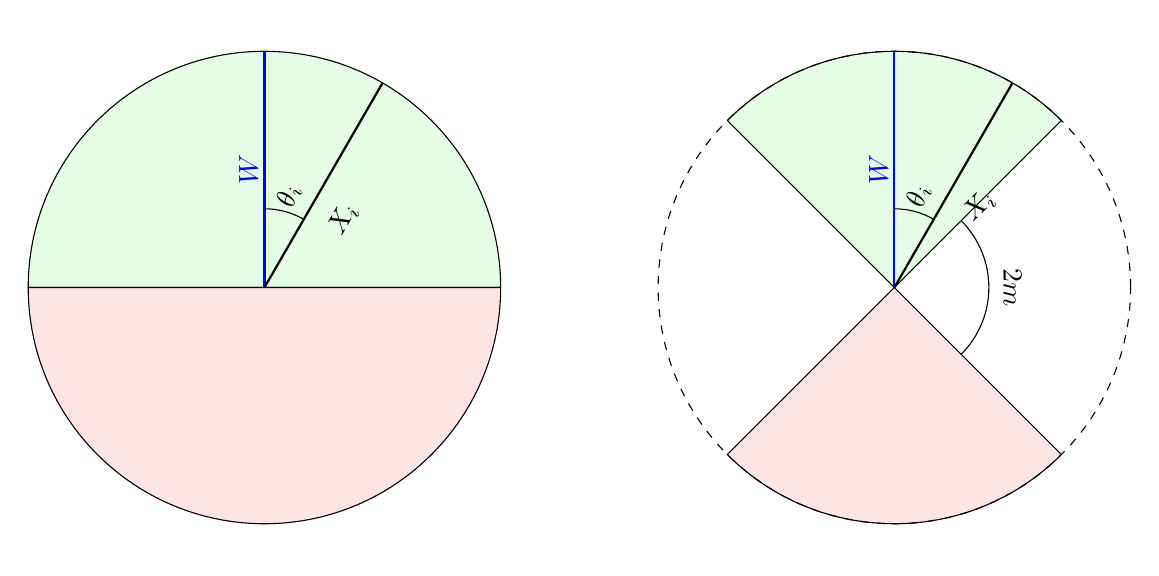
\begin{tikzpicture}
		% the origin
		\def\r{3}
		\def\rad{0.707106}
		

		%\draw[help lines] (-2,-4) grid (+2,+4);
		
		\draw[fill=green!10] (-4,0) -- (-4+\r,0) arc[start angle=0, end angle=180,radius=\r cm] -- (-4,0);
		
		\draw[thick,blue] (-4,0) -- (-4,\r);
		\node[color=blue , rotate=90] at (-4.2,1.5) {$W$};
		\node[color=black , rotate=60] at (-4+\r/3,\r * 0.8660/3) {$X_i$};
	%	\draw[color=blue] at (-4,2) {\texttt{$W$}};
		\draw (-4,1) arc [start angle=90, end angle=60,radius=1 cm] ;
		\node[color=black , rotate=75] at (-4+1.2*0.2588,1.2*0.9659) {$\theta_i$};
		%\draw (-4+0.5,0.8660) arc [start angle=60, end angle=90,radius=1 cm] (-4,1);
		\draw[thick,black] (-4,0) -- (-4+\r/2,\r * 0.8660);
		\draw[fill=red!10] (-4,0) -- (-4-\r,0) arc[start angle=180, end angle=360,radius=\r cm] -- (-4,0);
		
		\draw[fill=green!10] (4,0) -- (4+\r*\rad,\r*\rad) arc[start angle=45, end angle=135,radius=\r cm] -- (4,0);
		
		\draw[thick,blue] (+4,0) -- (+4,\r);
		\node[color=black , rotate=44] at (4+1.5*0.7193,0.694*1.5) {$X_i$};
		\node[color=blue , rotate=90] at (3.8,1.5) {$W$};
		\draw[thick,black] (4,0) -- (4+\r/2,\r * 0.8660);
		\draw[fill=red!10] (4,0) -- (4-\r*\rad,-\r*\rad) arc[start angle=225, end angle=315,radius=\r cm] -- (4,0);
		
			\draw (4,1) arc [start angle=90, end angle=60,radius=1 cm] ;
		\node[color=black , rotate=75] at (4+1.2*0.2588,1.2*0.9659) {$\theta_i$};
		
		\draw (5.2,0) arc [start angle=0, end angle=45,radius=1.2 cm] ;
		\draw (5.2,0) arc [start angle=0, end angle=-45,radius=1.2 cm] ;
		\node[color=black , rotate=270] at (5.5,0) {$2m$};
		\draw[dashed] (4,0) circle (\r cm);
		%\draw[thick]
		
		
		%\draw[dashed,red] (-3.5,0) circle (3cm) 
		
		%\draw (1,2) coordinate(a) circle (2pt);
	\end{tikzpicture}

	\caption{مقایسه تابع هزینه
	\lr{BCE} 
	کلاسیک با نسخه‌ی حاشیه‌دار
	\lr{ARCB} }
\label{fig:arcb}
\end{figure}
	

\section{تابع هزینه بر اساس شناسه‌ی شخص}
در دیتاست‌های موجود در حوزه کشف تقلب در چهره، برای هر فرد چند نمونه‌ی زنده و چند نمونه تقلبی وجود دارد. یعنی یک فرد که از چهره او برای جمع‌آوری داده استفاده شده است نمونه فیلم زنده و تقلبی او ضبط شده است. در ویدیو واقعی و تقلبی فرد در دیتاست یک ویژگی ظاهری یکسان شامل مشخصه‌های چهره‌ی وی وجود دارد که این مشخصه‌ها با فرد دیگر متفاوت است. از طرفی در فرآیند آموزش شبکه مطلوب این است که شبکه به‌جای تمرکز روی ویژگی‌های ظاهری چهره‌ی افراد روی علائم مربوط به وجود یا عدم وجود تقلب در چهره تأکید داشته باشد.

از آنجا که عمده تصویر ورودی به شبکه شامل چهره و مشخصات چهره می‌شود شبکه برای نمونه‌های مختلف از یک فرد دچار چسبندگی به روی ویژگی‌های چهره او خواهد شد که این امر مطلوب نیست.       
بدین جهت در این بخش یک جریمه برای این مورد در تابع هزینه قرار داده می‌شود که هدف شبکه این باشد که به ویژگی‌های ظاهری افراد توجه نکند و توجه آن به ویژگی‌های مربوط به تقلب باشد. فرض کنید بردار ویژگی خروجی قسمت استخراج ویژگی برای فرد $k$ ام با برچسب $l$ به‌صورت 
$X_k^l \in R^d , I \in \{0,1\}, K \in \{1,2,...,M\}$
 باشد.
در حین آموزش در هر گام تعداد دسته
\LTRfootnote{Batch size} $N$ 
فرض می‌شود. در میان این $N$ بردار ویژگی تعداد 
${N\choose 2}$
  جفت بردار ویژگی وجود دارد که در میان این تعداد جفت دو حالت مهم است.
  
  حالت اول زمانی که دو بردار ویژگی در جفت، متعلق به یک فرد ولی دارای برچسب مختلف هستند. یعنی 
  $k_1=k_2 , l_1 \ne l_2 $
  . در این حالت با توجه به اینکه مشخصه‌های ظاهری فرد که عمده تصویر ورودی است یکسان است لازم است که فاصله این دو نمونه بیشینه شود. با بیشینه کردن این فاصله شبکه مجبور می‌شود توجه خود را به‌جای مشخصه‌های ظاهری افراد به سمت ویژگی‌ای که تفاوت این دو نمونه است ببرد و این یعنی تفاوت برچسب این دو بردار ویژگی که یکی واقعی و یکی تقلبی است. 
  
  این حالت در شکل
\ref{fig:pid1}
  نشان داده شده است. در این شکل تصویر بالایی یک تصویر زنده و تصویر دومی تقلبی است. از آنجا که این دو تصویر شبیه هستند لذا خروجی بردارهای ویژگی آنها ممکن است که نزدیک هم باشند. بردارهای ویژگی متناظر با هر کدام در فضای $d$ بعدی نرمالایز شده نشان داده شده‌ است. لازم است که فاصله این دو بردار در این حالت بیشینه شود.
  
 \begin{figure}[ht]
 	%\centerline{\includegraphics[width=\linewidth]{pid1}}
 \centering

\begin{tikzpicture}
	\def\r{3}
	
	\def\h{2}
	\tikzstyle{connection}=[ultra thick,every node/.style={sloped,allow upside down},draw=\edgecolor,opacity=0.7]
	\node[canvas is zy plane at x=0] (im1) at (-5,\h,0)
	{\includegraphics[width=3cm,height=3cm]{p1-r.png}};
	\draw[->,thick,green] (-4.5,\h) -- (-4,\h);
	\node[canvas is zy plane at x=0] (im1) at (-5,-\h,0)
	{\includegraphics[width=3cm,height=3cm]{p1-f.png}};
	\draw[->,thick,red] (-4.5,-\h) -- (-4,-\h);
	%\draw [color=black]
	%(img) node[anchor=south] at (-5,-3){\texttt{Input Face}};
	%\draw[connection] 
	
	\node[rectangle,
	draw = orange!80,
	text = black,
	fill = orange!20,
	rotate=270,
	trapezium stretches = true,
	minimum width = 3cm, 
	minimum height = 0.75cm] (t) at (-3.6,\h) {$LBP_{tr}$};
	
	\node[rectangle,
	draw = orange!80,
	text = black,
	fill = orange!20,
	rotate=270,
	trapezium stretches = true,
	minimum width = 3cm, 
	minimum height = 0.75cm] (t) at (-3.6,-\h) {$LBP_{tr}$};
	
	\draw[->,thick,green] (-3.2,\h) -- (-2.7,\h);
	\node[trapezium,
	draw = blue!80,
	text = black,
	fill = teal!20,
	rotate=270,
	trapezium stretches = true,
	minimum width = 1.5cm, 
	minimum height = 2cm] (t) at (-1.7,\h) {\small \lr{EfficientNet}};
	
	\draw[->,thick,red] (-3.2,-\h) -- (-2.7,-\h);
	\node[trapezium,
	draw = blue!80,
	text = black,
	fill = teal!20,
	rotate=270,
	trapezium stretches = true,
	minimum width = 1.5cm, 
	minimum height = 2cm] (t) at (-1.7,-\h) {\small \lr{EfficientNet}};
	
	\draw[->,thick,green] (-0.7,\h) -- (-0.2,\h);
	\draw[->,thick,red] (-0.7,-\h) -- (-0.2,-\h);
	
	\pic[draw=red!80, fill=red!20] (FF) at (0.25,\h) {cube={0.25/1.2/0.25/0.25}};
	\node[color=black, rotate=270,] at (0.25,\h) {\small
		\lr{Feature Vector}};
	\draw[->,thick,green] (0.55,\h) -- (1.05,\h);
	\pic[draw=red!80, fill=red!20] (FN) at (1.45,\h) {cube={0.25/1.2/0.25/0.25}};
	\node[color=black, rotate=270,] at (1.45,\h) {\small
		$L_2\;Norm$};
	
	\pic[draw=red!80, fill=red!20] (FF) at (0.25,-\h) {cube={0.25/1.2/0.25/0.25}};
	\node[color=black, rotate=270,] at (0.25,-\h) {\small
		\lr{Feature Vector}};
	\draw[->,thick,red] (0.55,-\h) -- (1.05,-\h);
	\pic[draw=red!80, fill=red!20] (FN) at (1.45,-\h) {cube={0.25/1.2/0.25/0.25}};
	\node[color=black, rotate=270,] at (1.45,-\h) {\small
		$L_2\;Norm$};
	
	
	\draw (4, 0) node[circle, fill, inner sep=1] (orig) {};
	% Sphere
	
	
	% Axes
	\draw[->] (orig) -- ++(-\r/2, -\r/1.5) node[below] (x1) {$i_1$};
	\draw[->] (orig) -- ++(\r, 0) node[right] (x2) {$i_2$};
	\draw[->] (orig) -- ++(0, \r) node[above] (x3) {$i_d$};
	
	\draw (5, 2) node[circle, fill,green, inner sep=2,above] (p1r) {};
	
	\draw (6, 1) node[circle, fill,red, inner sep=2,above] (p1f) {};
	
	\draw [color=black]
	(p1r) node[anchor=east] {\texttt{$X_{k_1}^{l_1}$}}
	(p1f) node[anchor=west] {\texttt{$X_{k_2}^{l_2}$}};
	\draw [->,green,thick] (1.75,+\h) to [out=0,in=90] (p1r.north);
	
	\draw [->,red,thick] (1.75,-\h) to [out=0,in=-90] (p1f.south);
	
	
	\draw[<->,thick] (p1r) to (p1f) ;
	
	\node[color=black] at (5.75,-\h) {\lr{Normalized space $R^d$}};
	
	%\draw [->,thick] (2.4,-1.6) to [out=-90,in=90] (pi.north); 		
	
\end{tikzpicture}
 
 	\caption{حالتی که دو نمونه متعلق به یک شخص ولی یکی واقعی و دیگری تقلبی است}
 	\label{fig:pid1}
 \end{figure}

پس در حالت اول هدف شبکه به‌صورت رابطه
\ref{eq:pid1obj}
است.
\begin{equation}\label{eq:pid1obj}
	\max_{\Theta} {d( X_{k_1}^{l_1},X_{k_2}^{l_2} )} = \min_{\Theta}{\max(0,M-d( X_{k_1}^{l_1},X_{k_2}^{l_2} ))}
\end{equation}

که در آن 
$\Theta$
 مجموعه وزن‌های شبکه را نشان می‌دهد و تابع $d$ فاصله اقلیدسی بین دو بردار ویژگی نرمالایز شده است و به‌صورت رابطه 
\ref{eq:dfunc}
  تعریف می‌شود.
  \begin{equation}\label{eq:dfunc}
  	d(X_1,X_2) = ||\frac{X_1}{||X_1||}-\frac{X_2}{||X_2||}||
  \end{equation}

از آنجا که باید در بهینه‌سازی تابع هزینه کمینه شود بیشینه‌سازی فاصله دو بردار ویژگی معادل کمینه سازی مقدار 
$\max(0,M-d( X_{k_1}^{l_1},X_{k_2}^{l_2} ))$
 خواهد بود. در این رابطه $M$ یک هایپر پارامتر است که در صورتی که فاصله دو بردار ویژگی از این مقدار بیشتر باشد مقدار خروجی صفر خواهد بود و در صورتی که کمتر باشد میزان فاصله تا این مقدار $M$ به عنوان مقدار هزینه خواهد بود.
با توجه به نامساوی رابطه
\ref{eq:ne}
بیشترین فاصله‌ای که دو بردار ویژگی در فضای نرمالایز شده خواهند داشت عدد 2 خواهد بود و در پیاده سازی این تابع هزینه مقدار $M$ عدد 2 در نظر گرفته شده است.
  \begin{equation}\label{eq:ne}
	||\frac{X_1}{||X_1||}-\frac{X_2}{||X_2||}|| \le ||\frac{X_1}{||X_1||}||+||\frac{X_2}{||X_2||}||   \to d(X_1,X_2) \le 2
\end{equation}

حالت دوم زمانی که دو بردار ویژگی در جفت دارای یک برچسب ولی متعلق به اشخاص مختلفی هستند. به بیان ریاضی یعنی  
  $k_1 \ne k_2 , l_1 = l_2 $
. در این حالت با توجه به تفاوت مشخصه‌های ظاهری اشخاص این دو بردار ویژگی ممکن است فاصله محسوسی در فضای ویژگی داشته باشند. در این حالت مطلوب این است که فاصله این دو بردار ویژگی کم شود. در این صورت شبکه مجبور خواهد شد که به‌گونه‌ای از تصویر ویژگی انتخاب کند که فاصله این دو بردار ویژگی کم باشد و با رسیدن به این هدف ویژگی‌های استخراج شده بیشتر روی ویژگی‌های کشف تقلب تا ویژگی‌های ظاهری افراد تأکید دارند.

در شکل
\ref{fig:pid2}
این حالت نشان داده شده است. در این مثال دو تصویر ورودی هر دو از نوع تقلبی هستند ولی متعلق به اشخاص مختلفی هستند. از آنجا که دو فرد ویژگی‌های ظاهری متفاوتی دارند ممکن است فاصله بردارهای ویژگی متناظر با آن‌ها فاصله محسوسی داشته باشد. در این حالت کمینه کردن این فاصله مد نظر است. 
 \begin{figure}[ht]
	%\centerline{\includegraphics[width=\linewidth]{pid2}}
	 \centering
	
	\begin{tikzpicture}
		\def\r{3}
		
		\def\h{2}
		\tikzstyle{connection}=[ultra thick,every node/.style={sloped,allow upside down},draw=\edgecolor,opacity=0.7]
		\node[canvas is zy plane at x=0] (im1) at (-5,\h,0)
		{\includegraphics[width=3cm,height=3cm]{p1-r.png}};
		\draw[->,thick,green] (-4.5,\h) -- (-4,\h);
		\node[canvas is zy plane at x=0] (im1) at (-5,-\h,0)
		{\includegraphics[width=3cm,height=3cm]{p2-r.png}};
		\draw[->,thick,red] (-4.5,-\h) -- (-4,-\h);
		%\draw [color=black]
		%(img) node[anchor=south] at (-5,-3){\texttt{Input Face}};
		%\draw[connection] 
		
		\node[rectangle,
		draw = orange!80,
		text = black,
		fill = orange!20,
		rotate=270,
		trapezium stretches = true,
		minimum width = 3cm, 
		minimum height = 0.75cm] (t) at (-3.6,\h) {$LBP_{tr}$};
		
		\node[rectangle,
		draw = orange!80,
		text = black,
		fill = orange!20,
		rotate=270,
		trapezium stretches = true,
		minimum width = 3cm, 
		minimum height = 0.75cm] (t) at (-3.6,-\h) {$LBP_{tr}$};
		
		\draw[->,thick,green] (-3.2,\h) -- (-2.7,\h);
		\node[trapezium,
		draw = blue!80,
		text = black,
		fill = teal!20,
		rotate=270,
		trapezium stretches = true,
		minimum width = 1.5cm, 
		minimum height = 2cm] (t) at (-1.7,\h) {\small \lr{EfficientNet}};
		
		\draw[->,thick,red] (-3.2,-\h) -- (-2.7,-\h);
		\node[trapezium,
		draw = blue!80,
		text = black,
		fill = teal!20,
		rotate=270,
		trapezium stretches = true,
		minimum width = 1.5cm, 
		minimum height = 2cm] (t) at (-1.7,-\h) {\small \lr{EfficientNet}};
		
		\draw[->,thick,green] (-0.7,\h) -- (-0.2,\h);
		\draw[->,thick,red] (-0.7,-\h) -- (-0.2,-\h);
		
		\pic[draw=red!80, fill=red!20] (FF) at (0.25,\h) {cube={0.25/1.2/0.25/0.25}};
		\node[color=black, rotate=270,] at (0.25,\h) {\small
			\lr{Feature Vector}};
		\draw[->,thick,green] (0.55,\h) -- (1.05,\h);
		\pic[draw=red!80, fill=red!20] (FN) at (1.45,\h) {cube={0.25/1.2/0.25/0.25}};
		\node[color=black, rotate=270,] at (1.45,\h) {\small
			$L_2\;Norm$};
		
		\pic[draw=red!80, fill=red!20] (FF) at (0.25,-\h) {cube={0.25/1.2/0.25/0.25}};
		\node[color=black, rotate=270,] at (0.25,-\h) {\small
			\lr{Feature Vector}};
		\draw[->,thick,red] (0.55,-\h) -- (1.05,-\h);
		\pic[draw=red!80, fill=red!20] (FN) at (1.45,-\h) {cube={0.25/1.2/0.25/0.25}};
		\node[color=black, rotate=270,] at (1.45,-\h) {\small
			$L_2\;Norm$};
		
		
		\draw (4, 0) node[circle, fill, inner sep=1] (orig) {};
		% Sphere
		
		
		% Axes
		\draw[->] (orig) -- ++(-\r/2, -\r/1.5) node[below] (x1) {$i_1$};
		\draw[->] (orig) -- ++(\r, 0) node[right] (x2) {$i_2$};
		\draw[->] (orig) -- ++(0, \r) node[above] (x3) {$i_d$};
		
		\draw (5, 2) node[circle, fill,green, inner sep=2,above] (p1r) {};
		
		\draw (7, -1) node[circle, fill,red, inner sep=2,above] (p1f) {};
		
		\draw [color=black]
		(p1r) node[anchor=east] {\texttt{$X_{k_1}^{l_1}$}}
		(p1f) node[anchor=west] {\texttt{$X_{k_2}^{l_2}$}};
		\draw [->,green,thick] (1.75,+\h) to [out=0,in=90] (p1r.north);
		
		\draw [->,red,thick] (1.75,-\h) to [out=0,in=-180] (p1f.west);
		
		
		\draw[<->,thick] (p1r) to (p1f) ;
		
		\node[color=black] at (5.75,-\h) {\lr{Normalized space $R^d$}};
		
		%\draw [->,thick] (2.4,-1.6) to [out=-90,in=90] (pi.north); 		
		
	\end{tikzpicture}

	\caption{حالتی که دو نمونه متعلق به اشخاص مختلف ولی برچسب یکسان هستند}
	\label{fig:pid2}
\end{figure}
پس به بیان ریاضی در این حالت تابع هزینه به‌صورت رابطه
\ref{eq:pid2obj}
خواهد بود.
\begin{equation}\label{eq:pid2obj}
\min_{\Theta} {d( X_{k_1}^{l_1},X_{k_2}^{l_2} )} 
\end{equation}

  و در نهایت تابع هزینه بر اساس شناسه اشخاص موجود در دیتاست به‌صورت رابطه
\ref{eq:pid}
  خواهد بود. که در آن  
 $N_i$
   تعداد جفت نمونه‌ها با ویژگی برچسب یکسان و شخص متفاوت در دسته است و 
   $N_j$
       تعداد جفت نمونه با ویژگی برچسب متفاوت و شناسه یکسان است.
\begin{equation}\label{eq:pid}
  	L_{PiD} = \sum_{l_1 \ne l_2,k_1 \ne k_2}{\frac{1}{N_i}d( X_{k_1}^{l},X_{k_2}^{l})+\frac{1}{N_j}\max(0,M-d( X_{k}^{l_1},X_{k}^{l_2} ))}
\end{equation}

 نحوه تشکیل این تابع هزینه بدین صورت است که در هر گام آموزش از میان $N$ نمونه‌ی موجود در دسته تمامی جفت‌هایی که شرط شناسه متفاوت برچسب یکسان و یا شرط شناسه یکسان و برچسب متفاوت دارند انتخاب شده و فاصله اقلیدسی آن‌ها در رابطه
\ref{eq:pid}
 قرار داده می‌شود. این تابع هزینه وقتی کمینه شود شبکه به سمتی حرکت می‌کند که ویژگی‌های مطلوب برای کشف تقلب شناسایی شده و ویژگی‌هایی مرتبط به چهره افراد نادیده گرفته شود.
 
 تابع هزینه معرفی شده در این قسمت بر خلاف تابع هزینه
 \lr{ARCB}
 وظیفه‌ی طبقه‌بندی ندارد و تنها به عنوان یک نقش کمکی در کنار طبقه‌بندی کمک می‌کند. لذا هرچند که تابع هزینه 
  \lr{ARCB}
  به تنهایی قابل استفاده است اما تابع هزینه مبتنی بر شناسه‌ی اشخاص به تنهایی قابل استفاده نیست. این تابع یک تابع هزینه متریک است که با استفاده از شناسه اشخاص محدودیت خاصی روی فاصله‌ی جفت نمونه‌های خاص ارائه می‌کند. تابع هزینه متریک به صورت غیر مستقیم باعث افزایش دقت طبفه‌بندی و بهبود قابلیت تعمیم‌پذیری شبکه خواهد شد. در واقع این تابع هزینه باعث می‌شود که شبکه‌ی استخراج ویژگی به نحوی عمل کند که بردار‌های ویژگی به نحو مناسبی قرار بگیرند که دقت طبقه‌بندی بیشتر شود و شبکه ویژگی‌های اساسی برای تقلب را فارغ از ویژگی‌های ظاهری افراد استخراج کند. لازم به ذکر است که ایده استفاده از تابع هزینه متریک در کنار طبقه‌بندی روشی کارآمد است که در حوزه کشف تقلب در چهره نیز با فرمول‌بندی‌های مختلف استفاده شده است
\cite{shao2019multi,jia2020single,feng2020learning,perez2019deep,tu2020learning,xu2021improving}.
اما تابع هزینه پیشنهادی در این پایان‌نامه از شناسه اشخاص برای انتخاب جفت نمونه استفاده می‌کند که از این نظر با روش‌های قبلی متفاوت است.
  
  در نهایت تابع هزینه کلی برای آموزش شبکه شامل ترکیب خطی از دو تابع هزینه‌ی معرفی شده و به‌صورت رابطه
\ref{eq:ltot}
 خواهد بود. که در آن 
 $\lambda$
   هایپر پارامتر است.
\begin{equation}\label{eq:ltot}
	L_{overal} = L_{ArcB} + \lambda L_{PiD}
\end{equation}

\section{مقایسه‌ی روش پیشنهادی با پژوهش‌های قبلی}
ایده استفاده از 
\lr{LBP}
در مقایسه با سایر روش‌های کلاسیک اهمیت ویژه‌ای در حوزه کشف تقلب دارد
\cite{maatta2011face,chingovska2012effectiveness,freitas2012lbp,rehman2020enhancing,li2019face,yu2020searching,zhang2020face}.
روش \lr{LBP} قابل آموزش در این پژوهش، در مقایسه با روش‌هایی که از ترکیب کانولوشن و عملگر \lr{LBP} استفاده کرده‌اند
\cite{li2019face,rehman2020enhancing}
از این نظر متفاوت است که در روش‌های قبلی عملگر \lr{LBP} به‌صورت ایستا و بدون پارامتر بوده است اما روش پیشنهادی، یک عملگر قابل آموزش است که دارای پارمترهای یادگیری می‌باشد و در طول آموزش این پارامترها با توجه به داده‌های آموزش بهینه خواهند شد.

در
\cite{juefei2017local} 
از ایده عملگر \lr{LBP} قابل آموزش برای کاهش تعداد وزن‌های شبکه استفاده شده است. در واقع روش
\cite{juefei2017local} 
روی خاصیت تنک بودن
\LTRfootnote{Sparsity}
 عملگر \lr{LBP} تمرکز کرده است و قسمتی از وزن‌های شبکه را به‌صورت ثابت و با الهام از عملگر \lr{LBP} در نظر گرفته است و با این روش تعداد وزن‌های قابل آموزش را در شبکه کاهش داده است و نشان داده است که سرعت اجرای شبکه بهبود می‌یابد و دقت شبکه افت کمی خواهد کرد. روش ارائه شده در این پایان‌نامه تعداد وزن‌ها را کم نمی‌کند و دارای فرمول بندی به‌گونه‌ای است که از تفاوت تمامی پیکسل‌های مجاور با پیکسل مرکزی استفاده شود.
رابطه ارائه شده در 
\cite{juefei2017local} 
 به‌صورت رابطه
\ref{eq:deeplocal}
  است. که در آن 
  $b_i^{st}$
  وزن‌های ثابت به‌صورت تنک هستند و 
  $V_{l,i}^t$
  پارامترهای قابل آموزش است.
\begin{equation}\label{eq:deeplocal}
	X_{l+1}^t=\sum_{i=1}^{m}{\sigma(\sum_{s}{b_i^{st}*X_l^s })V_{l,i}^t}
\end{equation}

در 
\cite{yu2020searching}
نیز عملگر کانولوشن با الهام از عملگر \lr{LBP} تغییر داده شده است به گونه که در رابطه نهایی وزن متفاوتی به پیکسل مرکزی پنجره کانولوشن داده می‌شود و اعمال تابع غیرخطی بیرون مجموع‌گیری است. که به کلی از نظر فرمول بندی با عملگر ارائه شده در این پایان‌نامه متفاوت است. 
\begin{equation}\label{eq:central-dif4}
	y(p_0) = \sum_{p \in R} {w(p_n).x(p_0+p_n)} +
	\theta(-x(p_0))\sum_{p \in R}{w(p_n)}
\end{equation}




 

  




